\subsection{M.PC.8 - Efficienza temporale}
\begin{figure}[H]
    \centering
    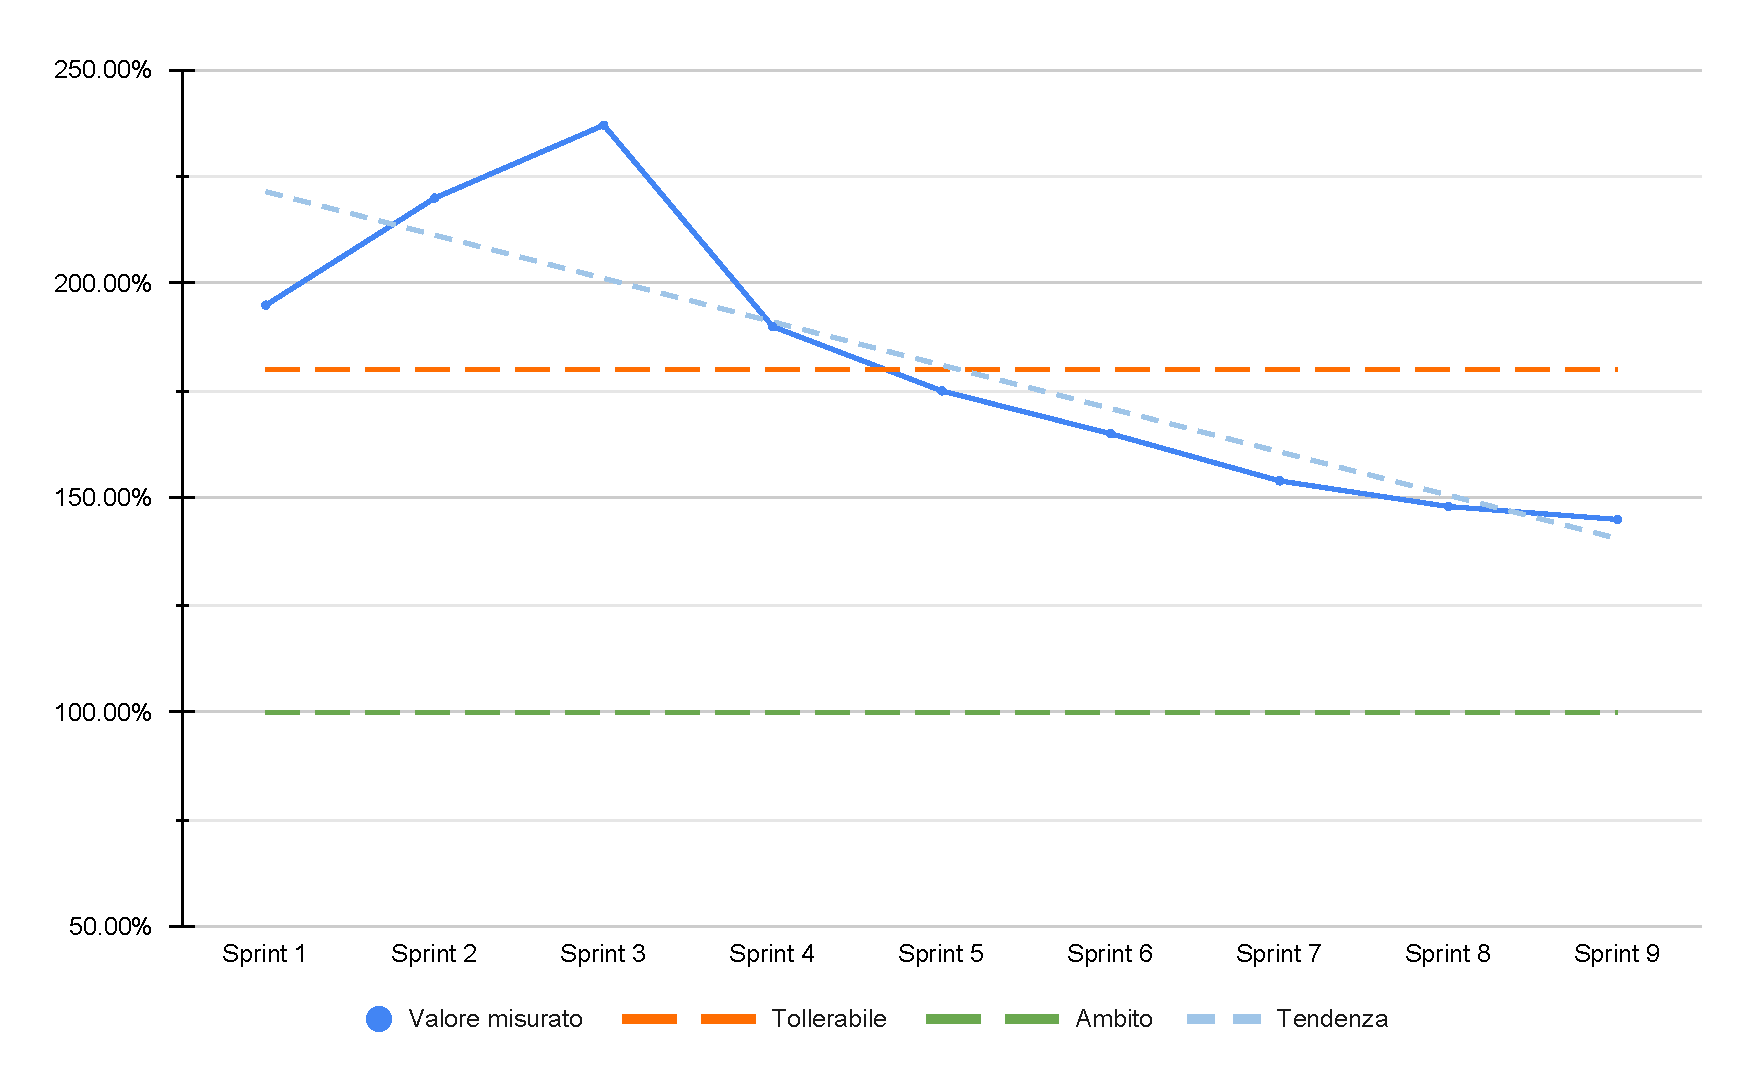
\includegraphics[width=\textwidth]{assets/efficienza_temporale.pdf}
    \caption{M.PC.8 - Efficienza temporale}
\end{figure}

\par Il grafico mostra un'iniziale sotto-performance rispetto alle aspettative, seguita da un miglioramento significativo nel corso del tempo. All'inizio del periodo monitorato, il gruppo impiegava un numero di ore che non si traduceva completamente in ore produttive, indicando possibili inefficienze o adattamenti iniziali alla parte di formazione e ricerca di strumenti. Tuttavia, con il passare degli \glossario{sprint}, si osserva un miglioramento costante dell'efficienza temporale. Possibili fattori di questo miglioramento sono l'inclusione di ottimizzazione dei processi, l'introduzione di nuovi strumenti o tecnologie, e un aumento della familiarità e della coesione del team.
In conclusione, il grafico dell'efficienza temporale testimonia un percorso di miglioramento da un inizio con prestazioni inferiori alle attese a un successivo riallineamento e superamento di queste aspettative. Questo evidenzia non solo una crescita numerica, ma anche un'adattabilità e una capacità di apprendimento del gruppo nel massimizzare l'uso delle proprie risorse per raggiungere risultati produttivi.
